\section{Hands-on experience}


% What did you choose to experiment with and why?

A more classic machine learning approach has been chosen to partially replicate the study. An extremely randomised decision tree (or Extra-Tree) \cite{geurts_extremely_2006} model has been fit to perform fully automatic vascular segmentation on one of the datasets used in the study, the DRIVE dataset \cite{staal_ridge-based_2004}. This model has been chosen for its simplicity to implement using scikit-learn \cite{pedregosa_scikit-learn:_2011}.


% Explain your setup

The DRIVE dataset consists on 20 training samples and 20 test samples. Each sample has an asocciated mask corresponding to the circular field of view and manual segmentations by human experts (one for the training samples and two for the test samples).

The code used to run the experiments is available online\footnote{\href{https://github.com/fepegar/cast-coursework}{https://github.com/fepegar/cast-coursework}}. The 12 features used for classification are the 3 RGB channels, the 3 HSV channels, the 3 L*a*b* channels, a Frangi vesselness filter \cite{frangi_multiscale_1998}, a Sobel filter and a Laplacian filter. The model has been trained using different weights for the foreground (vessels) and background (rest) classes, since most of the masked pixels of each label image are part of the background (87\% $\pm$ 2\%). Predictions are saved as probabilities of foreground class and thresholded at 0.5 to create binary prediction images.


% Report the results you obtained. Negative results are also interesting

Figure \ref{fig:collage} shows the segmentation results for the samples with highest, median and lowest Dice scores between the probability maps thresholded at 0.5 and the first manual segmentation. Most of the false negatives are smaller vessels, and most of the false positives are noisy predictions of isolated images. In DRIU, most of the false negatives are small vessels that were segmented by only one of the annotators, while most of the false positives are borders around the thinner vessels.

\begin{figure}
  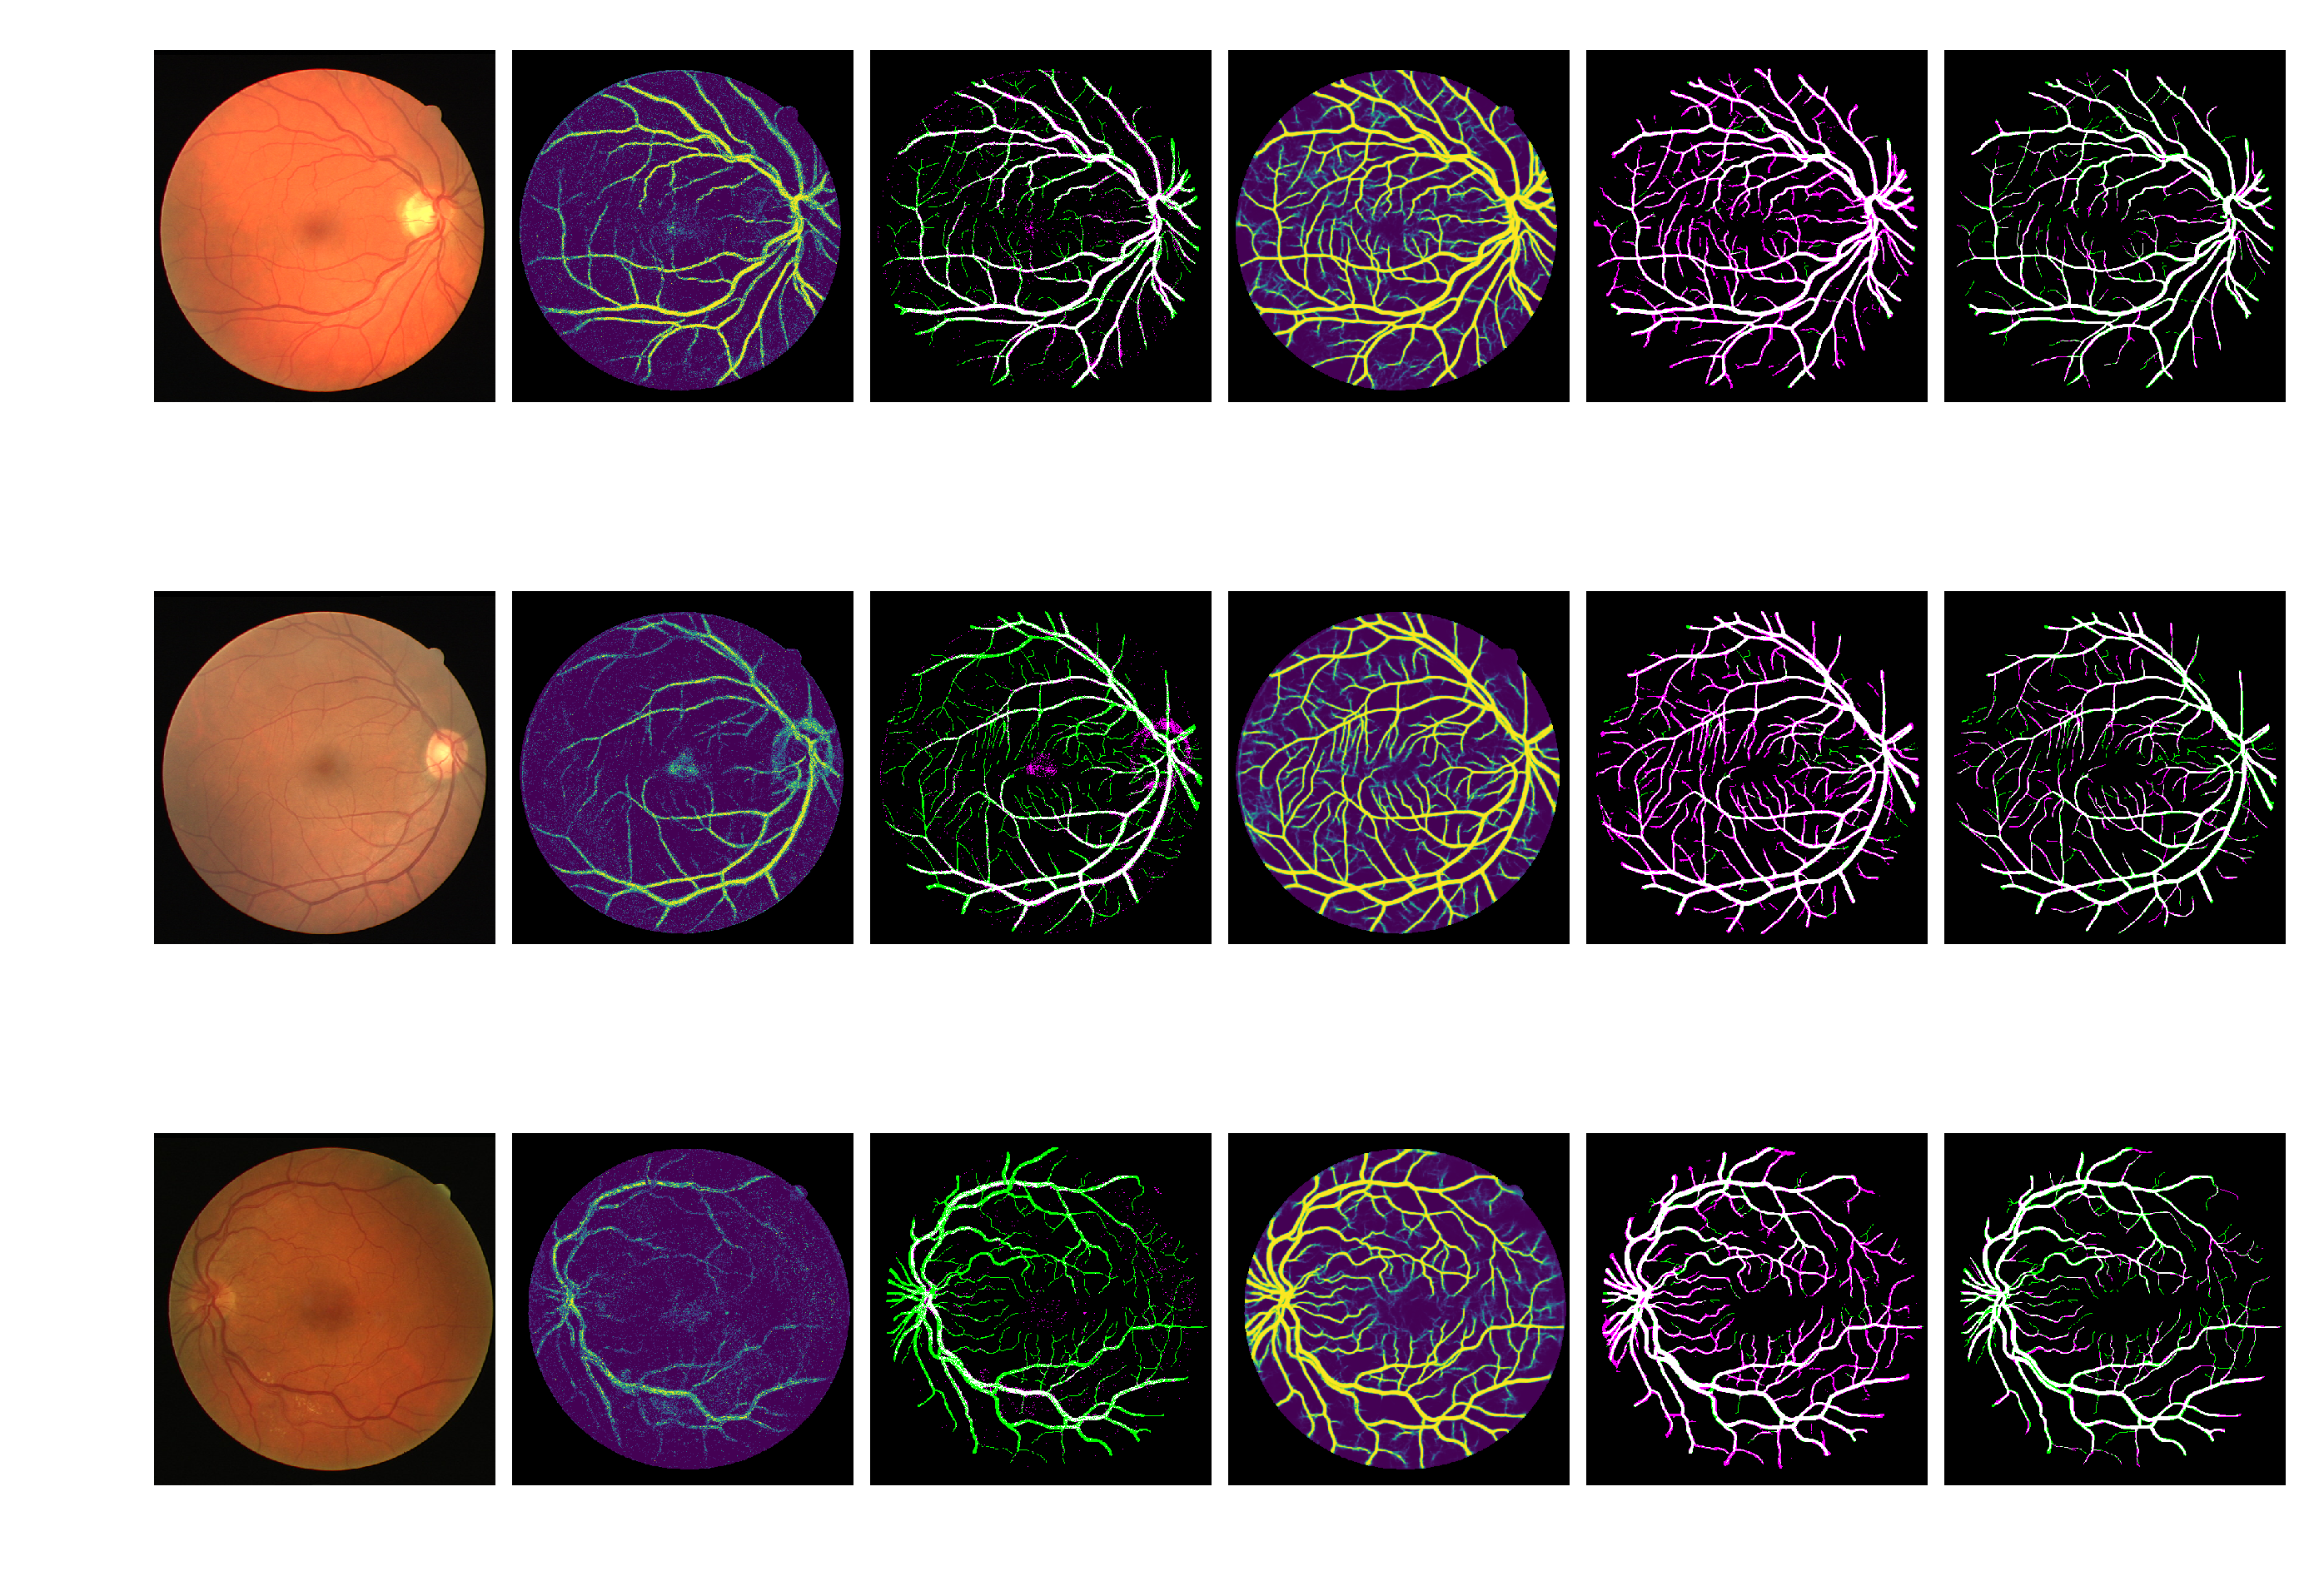
\includegraphics[width=\textwidth]{figures/collage}
  \caption{Results with highest (top), median (middle) and lowest (bottom) Dice scores using a 0.5 threshold. From left to right: acquired image of the retinal fundus; vessel probabilities using Extra-Trees; comparison of Extra-Trees thresholded probabilities to manual segmentation; vessel probabilities using DRIU; comparison of DRIU thresholded probabilities to manual segmentation; comparison of manual segmentation from first and second annotators. When comparing the binary images: first annotator is taken as groud truth; white pixels represent true positives; black pixels represent true negatives; magenta pixels represent false positives; and green pixels represent false negatives. The probability maps have been masked to show only the acquired field of view; higher lightness represents higher foreground probability} \label{fig:collage}
\end{figure}

Figure~\ref{fig:dice} shows all the Dice scores for both methods. DRIU presents higher scores for all cases.

\begin{figure}
  \centering
  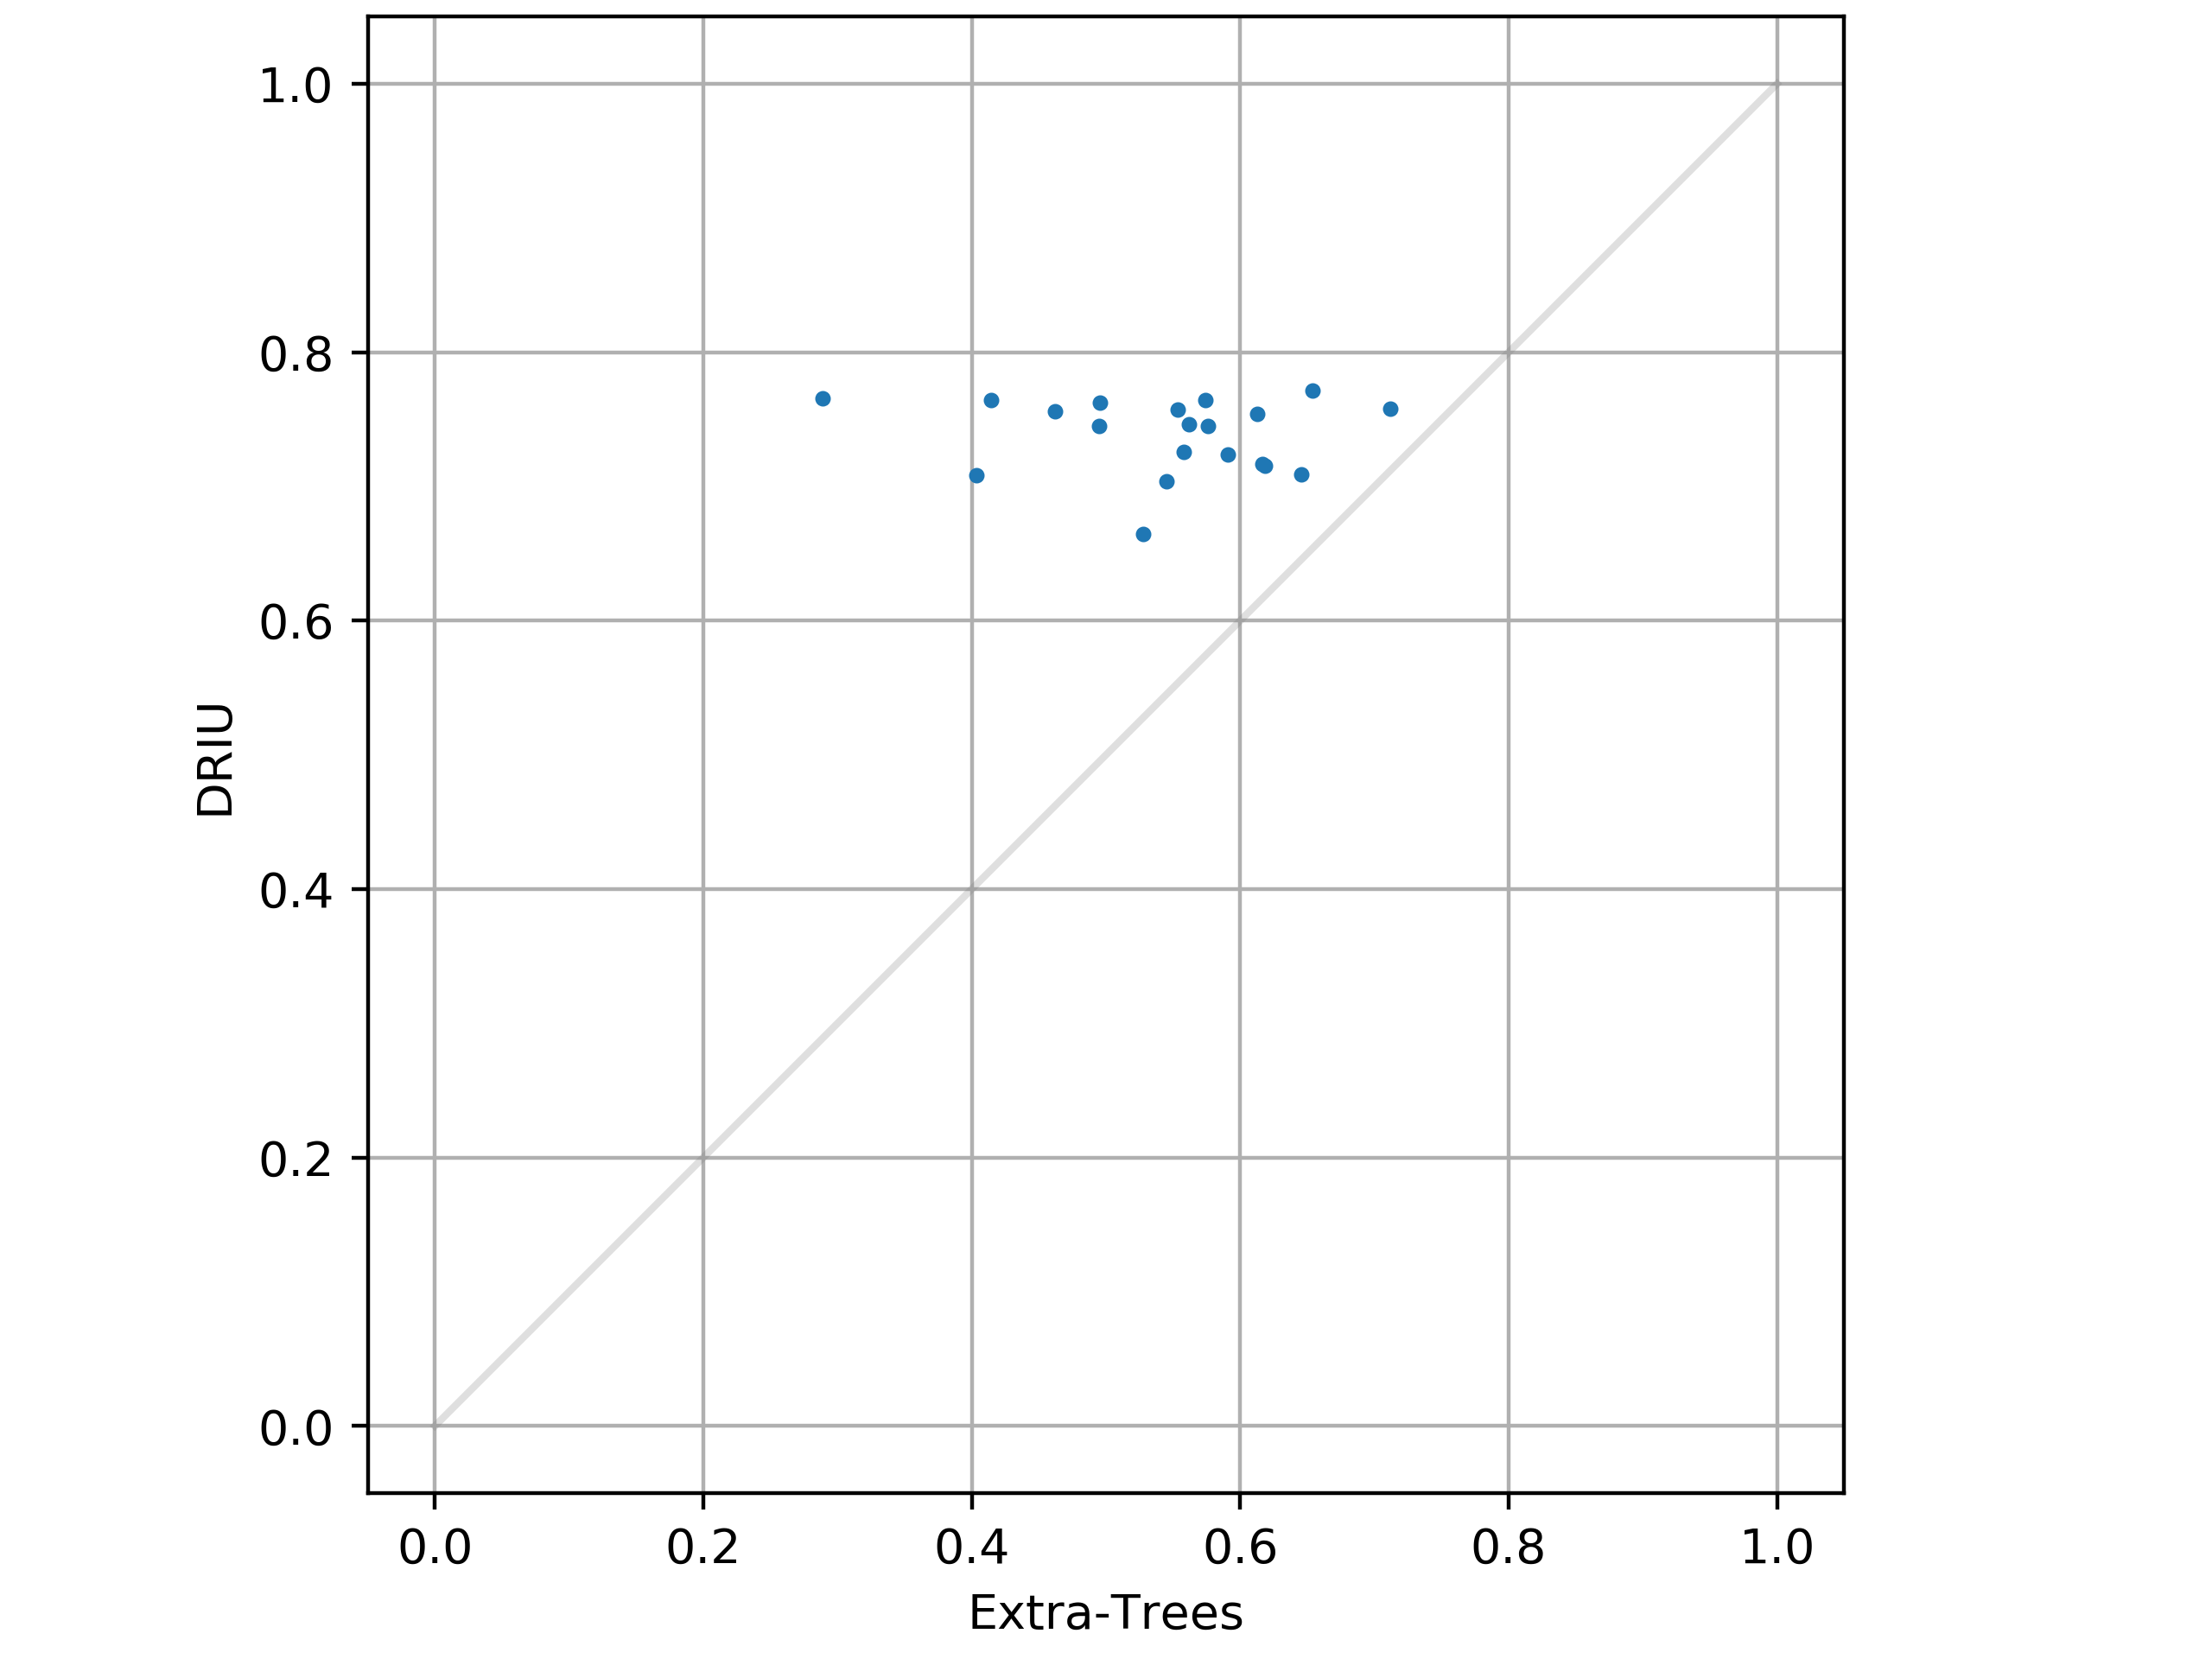
\includegraphics[width=0.8\textwidth]{figures/dices}
  \caption{Dice scores of both methods between probabilities thresholded at 0.5 and ground truth (first annotator).} \label{fig:dice}
\end{figure}

Figure~\ref{fig:importance} shows the importance of each pixel feature for the classification. As expected, the Frangi filter is the most relevant feature used by the algorithm, followed by the Sobel and Laplacian filters. Pixels in vessels seem to be much better represented by spatial filters than by colour features.

\begin{figure}
  \centering
  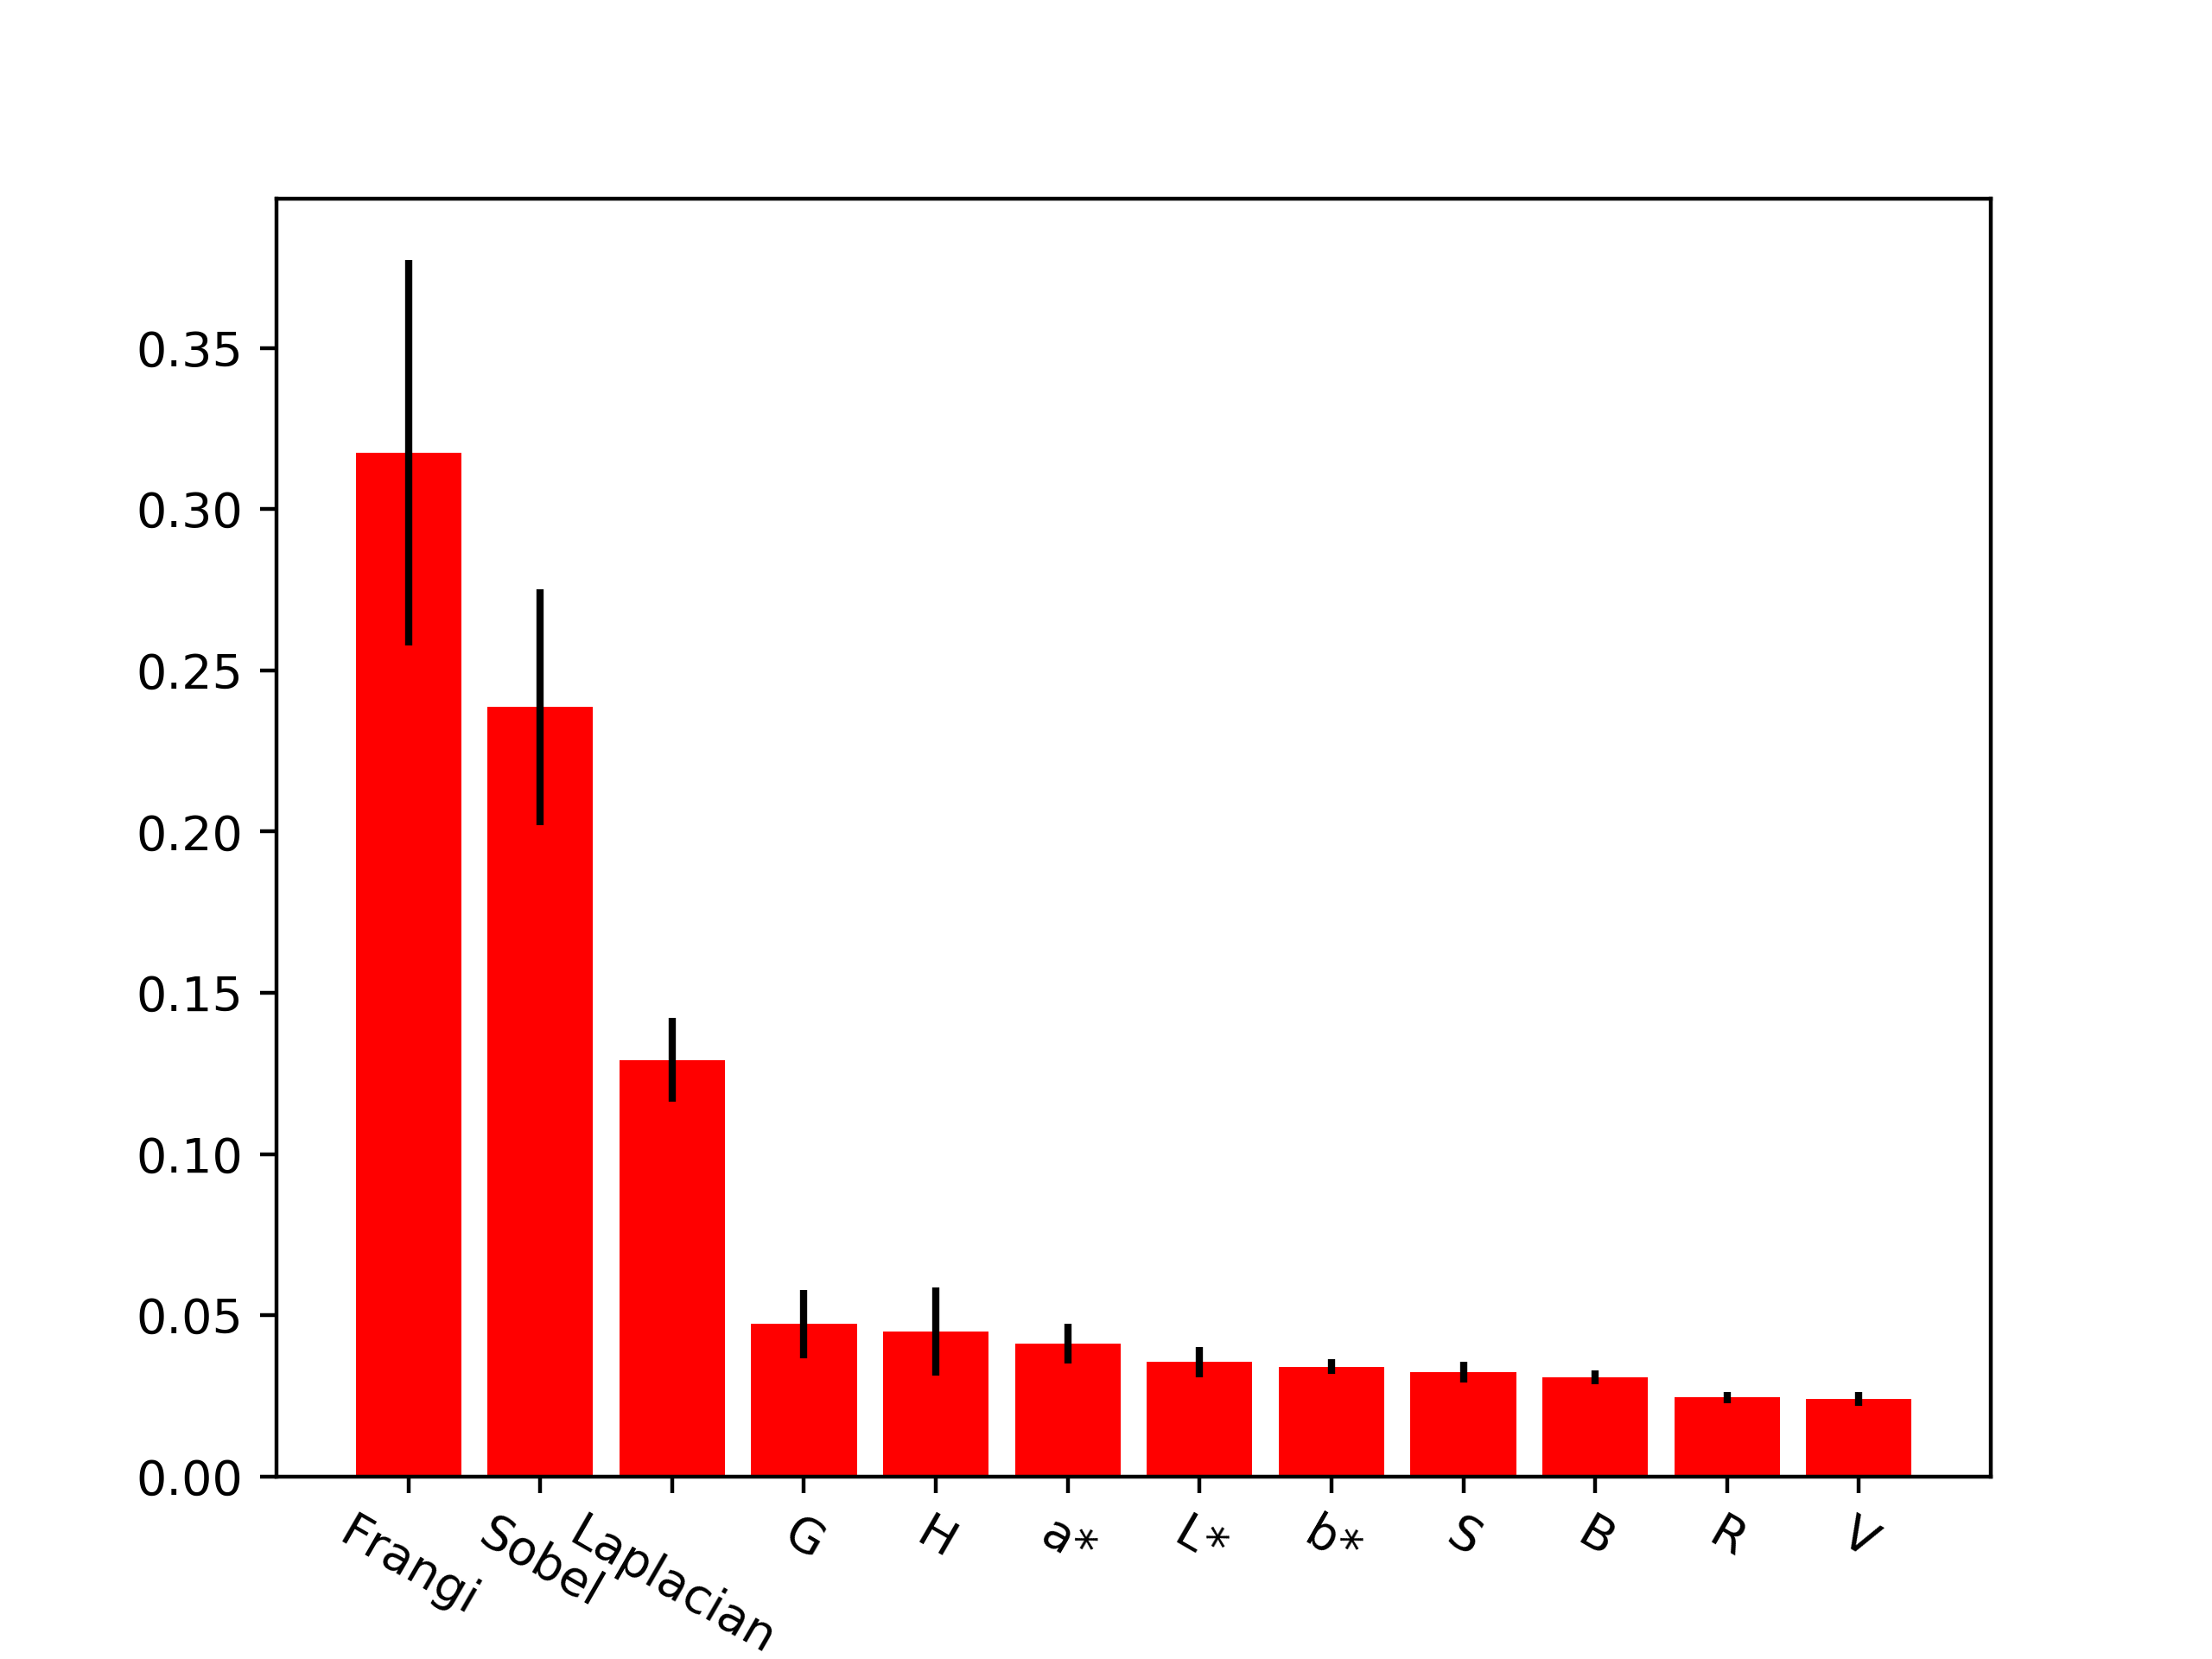
\includegraphics[width=0.8\textwidth]{figures/importances}
  \caption{Features importance for the forest, along with their inter-trees variability (standard deviation of the importance for each Extra-Trees estimator).} \label{fig:importance}
\end{figure}
